%From 관측계획서_ver5.tex
%Copyright ⓒ 2015  박승원(seungwonpark), Gyeonggi Science HighSchool for the Gifted. All rights reserved. Email : psw14041@gmail.com
\documentclass[11pt]{article}
\usepackage[left=25mm,right=25mm,top=30mm,bottom=30mm]{geometry}
\usepackage{amsmath} % math
\usepackage{amssymb} % math
\usepackage{graphicx} % to use \includegraphics{}
\usepackage{diagbox} % to make tables
\usepackage{kotex}
\begin{document}
	\begin{center}
		\Large 관측계획서 : 시간에 따른 별의 섬동(Scintillation) 경향성
		
		\Large Obsevation Plan : Graphing the Amount of Scintillation about time
		\normalsize
		\begin{flushright}
			과학영재학교 경기과학고등학교
			
			32nd 14041 박승원
		\end{flushright}
	\end{center}
	\tableofcontents
	\listoffigures
	\clearpage
	\section{연구 개요}
	
	관측천문을 하는 데에 있어서 별의 섬동(Scintillation)은 무시하지 못할 요소이다. Scintillation이란 천체를 관측하는 데에 있어서 상층 대기의 요동에 의해 빛의 경로가 휘어 별이 반짝여 보이는 현상으로, 직경이 작은 망원경일수록 심하게 나타난다.
	
	어떤 망원경을 이용하여 밝기 변화에 민감한 연구를 진행하기 위해서는 별의 섬동이 그 망원경이 설치된 지역에 맞게 수치적으로 DB화되어있어야 한다.
	\footnote{그 예시로 남극에 위치한 Dome C에서의 turbulence profile을 제공하는 reference로서의 논문이 있다.\cite{ant_scin}}
	하지만, 수원시 장안구 송죽동에 맞는 별의 섬동 DB에 관한 연구가 없었다.
	
	나는 이 관측을 통해 경기도 수원시 장안구 송죽동
	\footnote{위도 37.3도, 경도 127.0도}
	에 위치한 경기과학고등학교 천문대에서의 시간에 따른 섬동(Scintillation)의 정도를 구하고자 한다. 또한, 가능하다면 \textit{J. Osborn et al.}에 의한 새로운 Scintillation을 수치적으로나마 검증해 보고자 한다.
	
	\section{사용기기}
	
	망원경 : Celestron C-14. F ; 3910mm. f/11
	
	CCD : SBIG STX-16803 \cite{ccd}
	
	\section{관측개요}
	되도록 밝은 별을 촬영하고자 한다. 밝은 별을 촬영해야 짧은 노출 시간으로도 선명한 상을 얻을 수 있고, 찾기도 쉽기 때문이다. 노출 시간이 짧아야 scintillation이 더 잘 나타날 것으로 예상된다. 
	
	\subsection{이론적 배경 - 시간에 따른 Scintillation의 정도} \label{exp_1}
	
	Brian D.Warner의 \textquotedblleft A Practical Guide to Lightcurve Photometry and Analysis \textquotedblright 에 의하면 scintillation에 의한 분산 $\sigma$는 식 \ref{young}과 같이 계산된다.
	\begin{equation} \label{young}
	\sigma = 0.09 \cdot \frac{X^{1.5}}{D^{2/3}\sqrt{2\cdot t}} \cdot \exp{(-h/h_0)}
	\end{equation}
	
	$X$ = airmass = $\sec{\theta}$ where $\theta$ is the zenith angle of the observation
	
	$D$ = telescope aperture(cm)
	
	$t$= exposure duration(sec)
	
	$h$ = observatory elevation(cm)
	
	$h_0$ = atmospheric scale height
	
	식 \ref{young}는 1967년에 제창된 Young's Equation이다. 이 식의 0.09는 경험적인 값으로, McDonald 천문대에서 측정된 수치이다. 하지만, 어떠한 상황에 대해서도 Scintillation의 정도가 0.09와 같은 중간값과는 시간에 따라 차이가 있을 수 있다.\cite{Osborn} 1998년에 식 \ref{dravin}과 같은 Dravin's Equation이 제창되었다.
	
	\begin{equation} \label{dravin}
	\sigma = \sqrt{ 10.7\int_{0}^{\infty}{ \frac{C_n^2(h)h^2dh}{V_\perp} } } X^{7/4}D^{-2/3}t_{exp}^{-1/2}
	\end{equation}
	
	\subsection{시간에 따른 scintillation 분산 $\sigma$그래프 얻기}
	
	식 \ref{dravin}에 의하면 $\sigma$는 $1/\sqrt{t}$에 비례할 것으로 예상된다. 따라서 나는 동일한 시간대에 같은 별을 서로 다른 노출시간을 주어 가며 촬영해 보고, $\sigma - t$그래프를 그려 볼 것이다.
	어떤 임계치 $t_c$에 대해 $t>t_c$의 경우 scintillation이 더 이상 잘 나타나지 않을 것을 예상된다. 실험 데이터를 통해 $t_c$를 결정할 것이다.
	\ref{exp_1}절의 방법대로 $t_c$를 결정한 후, $t_c$, $t_c$보다 짧은 시간, $t_c$보다 긴 시간의 노출시간을 주어 같은 시간대에 같은 별을 서로 다른 세 노출시간으로 촬영해 볼 것이다.
	
	촬영할 별의 위치는 천정에 있는 것을 채택할 것이다. 천정에서의 대기에 의한 Scintillation을 촬영해야 우리 지역의 대기에 의한 효과만을 고려할 수 있기 때문이다.
	9월에 관측하게 될 경우 9월 23일 추분 기준으로 태양의 적경이 0h이며, 적위는 37.3도의 별들을 보게 된다.
	
	\section{Scintillation을 어떻게 구할 것인가?}
	
	\subsection{촬영 방법}
	기본적인 촬영 설정은 다음과 같다.
	\begin{flushleft}
		Exposure Preset : Find DSO 
		
		Filter Wheel : V
		
		Exposure Time : Manual
		
		Image Size : 4096*4096 (X Binning = 1)
		
		\begin{figure}[h]
			\begin{center}
				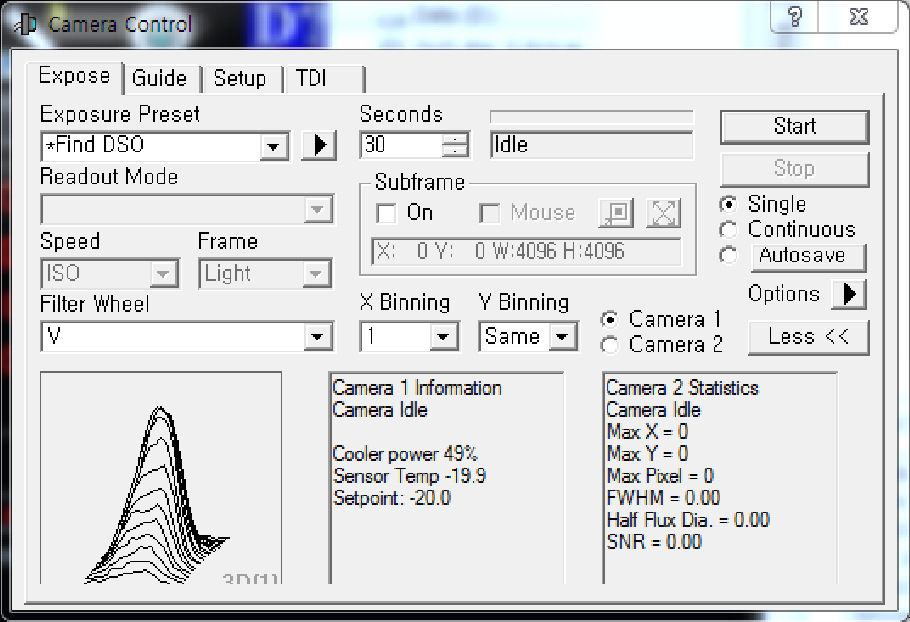
\includegraphics[scale=0.3]{camera_control_example.png}
				\caption{Maxim DL에서의 Camera Control 화면.}
				\label{camera_control}
			\end{center}
		\end{figure}
		
	\end{flushleft}
	
	\subsection{Simple Method - Data Reduction}
	
	\subsection{Speckle Imaging}
	
	이제 Scintillation을 어떻게 포착해 낼 것인가에 관해 논의할 것이다. 그에 관련한 사항으로 Speckle Imaging이 있다. \cite{speckle_img}
	
	\subsection{QVANTOS}
	
	Beam Splitter, 두 개의 광전자 증배관(PhotoMultipliers)과 Digital Correlator를 이용하여 Scintillation의 정도를 파악하는 방법이 있다. \cite{AISS.1}
	
	\begin{figure}[h]
		\begin{center}
			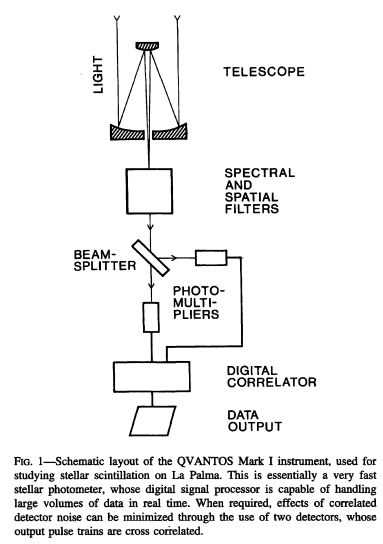
\includegraphics[scale=0.5]{QVANTOS.png}
			\caption{\textit{Dravins et al.}에서 소개된 QVANTOS 방법.}
			\label{QVANTOS}
		\end{center}
	\end{figure}
	
	\section{관측계획}
	\subsection{날씨}
	
	관측할 날을 정하기 위해 고려해야 할 가장 큰 점은, (당연하지만) 구름이 없어야 하며 달이 관측시간 내외에서 남중하는 날은 피해야 한다. 2015년 9~12월 중 보름달이 뜨는 날은 9월 28일, 10월 28일, 11월 26일, 12월 26일이다. 반면 달이 아예 뜨지 않는 날(삭)은 9월 13일, 10월 12일, 11월 11일, 12월 10일이다.
	
	\subsection{관측 횟수}
	
	관측 시 발생할 실수나 오류 등을 고려하고, 충분한 데이터를 얻기 위하여 관측은 3회정도 실시해야 할 것이다.
	
	\subsection{관측하는 날의 구체적 일정}
	
	- www.kma.go.kr\cite{kma}에서 날씨영상-위성-기본영상으로 구름이 적은지 확인. 적외영상으로 아시아 전체 모습도 확인할 것.
	
	- 정오 전까지 김혁 선생님(010-5536-0743)께 문자드리기
	
	- 오후 5시에 온도 안정화를 위해 돔을 미리 오픈해두고, 망원경과 CCD cooler를 켜놓는다.
	
	- 일몰 직후 Flat 보정용영상을 촬영한다. Flat은 Alt 60도 내외에서 SouthEast를 바라보며 25000$\sim$30000 ADU가 되도록 노출시간을 조정하며 동$\longrightarrow$서 1$\sim$2도 간격으로 5장 정도를 찍는다.
	
	- Flat 촬영 후 저녁식사.
	
	- 망원경의 한 지점을 잡아서 Sync.
	
	- 관측.
	
	- 마무리 : CCD warm up 이후 power off, dome close
	
	\subsection{일반적인 주의사항들}
	- Scintillation을 관측하기 위해 별의 떨림을 측정해야 하므로, 망원경의 떨림을 최소화해야 한다. 바람이 많이 부는 날은 피해야 하며, 망원경에 노출을 주고 있는 동안에는 몸의 동작을 삼가야 한다.
	
	\addcontentsline{toc}{section}{References}
	\begin{thebibliography}{00}
		
		\bibitem{Osborn}{Osborn, J., Föhring, D., Dhillon, V. S., \& Wilson, R. W. (2015). Atmospheric scintillation in astronomical photometry. Monthly Notices of the Royal Astronomical Society, \textbf{452}(2), 1707-1716.}
		
		\bibitem{ant_scin}{Kenyon, S. L., Lawrence, J. S., Ashley, M. C., Storey, J. W., Tokovinin, A., \& Fossat, E. (2006). Atmospheric Scintillation at Dome C, Antarctica: Implications for Photometryand Astrometry. Publications of the Astronomical Society of the Pacific, \textbf{118}(844), 924-932.}
		
		\bibitem{speckle_img}{Beavers, W., Dudgeon, D. E., Beletic, J. W., \& Lane, M. T. (1989). Speckle imaging through the atmosphere. Unknown, 1.}
		
		\bibitem{AISS.1}{D.Dravins, L.Lindegren, E.Mezey, A.T.Young, Astronomical Society of the Pacific \textbf{109}; 173-207, 1997 February}
		
		\bibitem{kma}{www.kma.go.kr (일출/일몰/월출/월몰시간 데이터)}
		
		\bibitem{ccd}{https://www.sbig.com/products/cameras/stx/stx-16803/}
		
	\end{thebibliography}
	
\end{document}